\documentclass[11pt]{article}
%%%%%%%%%%%%%%%%%%%%%%%%%%%%%%%%%%%%%%%%%%%%%%%%%%%%%%%%%%%%%%%
% DO NOT EDIT THIS FILE UNLESS YOU KNOW WHAT YOU ARE DOING!!! %
%%%%%%%%%%%%%%%%%%%%%%%%%%%%%%%%%%%%%%%%%%%%%%%%%%%%%%%%%%%%%%%

% Useful packages
\usepackage[]{authblk}
\usepackage{graphicx}
\usepackage{color}
\usepackage{longtable}
\usepackage{hanging}
\usepackage{indentfirst}
\usepackage{setspace}
\usepackage{enumitem}
\usepackage{verbatim}
\usepackage{upgreek}
\usepackage{framed}
\usepackage{textcomp}
\usepackage{url}
\usepackage{soul}
\usepackage{amsmath,amsfonts,amssymb,mathrsfs}
\usepackage{fancyhdr}
\usepackage[compact]{titlesec}
\usepackage[T1]{fontenc}
\usepackage{lmodern}
\usepackage[utf8]{inputenc}
\usepackage[]{listings}
%\usepackage{fontspec}
\usepackage{placeins}
\usepackage{epstopdf}
\usepackage[export]{adjustbox}
\usepackage{tikz}
\usepackage[breaklinks]{hyperref}
\usepackage[all]{hypcap}


% References
\usepackage[backend=bibtex,hyperref=true,citestyle=authoryear,bibstyle=authortitle,firstinits=true,terseinits=true,doi=false,url=false,eprint=false,maxbibnames=10,maxcitenames=2]{biblatex}
\DeclareCiteCommand{\cite}
  {\usebibmacro{prenote}}
  {\usebibmacro{citeindex}%
   \printtext[bibhyperref]{\usebibmacro{cite}}}
  {\multicitedelim}
  {\usebibmacro{postnote}}

\DeclareCiteCommand*{\cite}
  {\usebibmacro{prenote}}
  {\usebibmacro{citeindex}%
   \printtext[bibhyperref]{\usebibmacro{citeyear}}}
  {\multicitedelim}
  {\usebibmacro{postnote}}

\DeclareCiteCommand{\parencite}[\mkbibparens]
  {\usebibmacro{prenote}}
  {\usebibmacro{citeindex}%
    \printtext[bibhyperref]{\usebibmacro{cite}}}
  {\multicitedelim}
  {\usebibmacro{postnote}}

\DeclareCiteCommand*{\parencite}[\mkbibparens]
  {\usebibmacro{prenote}}
  {\usebibmacro{citeindex}%
    \printtext[bibhyperref]{\usebibmacro{citeyear}}}
  {\multicitedelim}
  {\usebibmacro{postnote}}

\DeclareCiteCommand{\footcite}[\mkbibfootnote]
  {\usebibmacro{prenote}}
  {\usebibmacro{citeindex}%
  \printtext[bibhyperref]{ \usebibmacro{cite}}}
  {\multicitedelim}
  {\usebibmacro{postnote}}

\DeclareCiteCommand{\footcitetext}[\mkbibfootnotetext]
  {\usebibmacro{prenote}}
  {\usebibmacro{citeindex}%
   \printtext[bibhyperref]{\usebibmacro{cite}}}
  {\multicitedelim}
  {\usebibmacro{postnote}}

\DeclareCiteCommand{\textcite}
  {\boolfalse{cbx:parens}}
  {\usebibmacro{citeindex}%
   \printtext[bibhyperref]{\usebibmacro{textcite}}}
  {\ifbool{cbx:parens}
     {\bibcloseparen\global\boolfalse{cbx:parens}}
     {}%
   \multicitedelim}
  {\usebibmacro{textcite:postnote}}

\newcommand{\citep}{\parencite}
\newcommand{\citet}{\textcite}
\defbibheading{relevref}[\refname]{\section*{Relevant References}}

\renewcommand{\postnotedelim}{\iffieldpages{postnote}{\addcolon}{\addcomma\space}} 
\DeclareFieldFormat{postnote}{#1} 

\DeclareFieldFormat[article, inbook, incollection, inproceedings, patent, thesis, unpublished]{title}{#1}
\DeclareFieldFormat[article, inbook, incollection, inproceedings, patent, thesis, unpublished]{journaltitle}{\mkbibemph{#1}\nopunct}
\DeclareFieldFormat[article, inbook, incollection, inproceedings, patent, thesis, unpublished]{volume}{{#1}\addcolon} %puts volume number in parens
%\DeclareFieldFormat[article, inbook, incollection, inproceedings, patent, thesis, unpublished]{year}{\mkbibparens{#1}\nopunct} %puts year in parens

\DeclareFieldFormat[article, incollection, patent, thesis, unpublished]{pages}{{\nopp#1}}

\DeclareFieldFormat{sentencecase}{\MakeSentenceCase{#1}}

\renewbibmacro*{title}{%
  \ifthenelse{\iffieldundef{title}\AND\iffieldundef{subtitle}}
    {}
    {\ifthenelse{\ifentrytype{article}\OR\ifentrytype{inbook}%
      \OR\ifentrytype{incollection}\OR\ifentrytype{inproceedings}%
      \OR\ifentrytype{inreference}}
      {\printtext[title]{%
        \printfield[sentencecase]{title}%
        \setunit{\subtitlepunct}%
        \printfield[sentencecase]{subtitle}}}%
      {\printtext[title]{%
        \printfield[titlecase]{title}%
        \setunit{\subtitlepunct}%
        \printfield[titlecase]{subtitle}}}%
     \newunit}%
  \printfield{titleaddon}}

\DefineBibliographyStrings{english}{% various adjustments to common bib entry strings
urlseen = {Accessed:},% What goes in front of the date a URL was accessed/retrieved etc.
editor = {(Ed)},%Ed – no dot, in brackets
editors = {(Eds)},% Eds – no dot, in brackets
byeditor = {(Ed.)}}% ‘Edited by’ for edited works

\DeclareNameAlias{default}{last-first}

\renewbibmacro{in:}{}

\renewbibmacro{publisher+location+date}{
  \iflistundef{publisher}
    {}
    {\printlist{publisher}%
       {\addcomma\space}%
      \iflistundef{location}
        {}
        {\printlist{location}}%
    }
}

\DeclareBibliographyDriver{article}{%
\usebibmacro{bibindex}%
\usebibmacro{begentry}%
\usebibmacro{author/translator+others}%
\newunit\newblock
\printfield{year}%
\setunit{\labelnamepunct}\newblock
\usebibmacro{title}%
\newunit
\printlist{language}%
\newunit\newblock
\usebibmacro{byauthor}%
\newunit\newblock
\usebibmacro{bytranslator+others}%
\newunit\newblock
\printfield{version}%
\newunit\newblock
%\usebibmacro{in:}% %mit in:
\usebibmacro{journal}%
\newunit\newblock
\printfield{volume}%
\newunit\newblock
\usebibmacro{byeditor+others}%
\newunit\newblock
\usebibmacro{note+pages}%
\newunit\newblock
\iftoggle{bbx:isbn}
{}%
\newunit\newblock
\usebibmacro{doi+eprint+url}%
\newunit\newblock
\usebibmacro{addendum+pubstate}%
\newunit\newblock
\usebibmacro{pageref}%
\usebibmacro{finentry}}

\DeclareBibliographyDriver{inproceedings}{%
\usebibmacro{bibindex}%
\usebibmacro{begentry}%
\usebibmacro{author/translator+others}%
\newunit\newblock
\printfield{year}%
\setunit{\labelnamepunct}\newblock
\usebibmacro{title}%
\newunit
\printlist{language}%
\newunit\newblock
\usebibmacro{byauthor}%
\newunit\newblock
\usebibmacro{bytranslator+others}%
\newunit\newblock
\printfield{version}%
\newunit\newblock
%\usebibmacro{in:}% %mit in:
\usebibmacro{booktitle}%
\newunit\newblock
\printfield{volume}%
\newunit\newblock
\usebibmacro{byeditor+others}%
\newunit\newblock
\usebibmacro{publisher+location+date}%
\newunit\newblock
\usebibmacro{note+pages}%
\newunit\newblock
\usebibmacro{pageref}%
\usebibmacro{finentry}}

\DeclareBibliographyDriver{book}{%
\usebibmacro{bibindex}%
\usebibmacro{begentry}%
\usebibmacro{author/translator+others}%
\newunit\newblock
\printfield{year}%
\setunit{\labelnamepunct}\newblock
\usebibmacro{title}%
\newunit
\printlist{language}%
\newunit\newblock
\usebibmacro{byauthor}%
\newunit\newblock
\usebibmacro{bytranslator+others}%
\newunit\newblock
%\usebibmacro{in:}% %mit in:
\usebibmacro{booktitle}%
\newunit\newblock
\printfield{volume}%
\newunit\newblock
\usebibmacro{publisher+location+date}%
\newunit\newblock
\usebibmacro{note+pages}%
\newunit\newblock
\usebibmacro{pageref}%
\usebibmacro{finentry}}




% Page margins
\setlength{\evensidemargin}{0in}
\setlength{\headheight}{0in}
\setlength{\headsep}{0in}
\setlength{\oddsidemargin}{-0.25in}
\setlength{\paperheight}{11in}
\setlength{\paperwidth}{8.5in}
\setlength{\tabcolsep}{0in}
\setlength{\textheight}{9in}
\setlength{\textwidth}{7in}
\setlength{\topmargin}{0in}
\setlength{\topskip}{0in}
\setlength{\voffset}{0in}
\parskip = 0.15in
\pagestyle{plain}
\setlength{\parindent}{0cm}

% No white space between list items
\setlist{nolistsep}

% Hyperlink setup
\hypersetup{colorlinks=true,linkcolor=linkscol,citecolor=citescol,urlcolor=urlscol}

% Settings for code blocks
\lstset{backgroundcolor=\color[rgb]{0.972,0.972,0.972},
    tabsize=4,
    rulecolor=,
        basicstyle=\scriptsize,
        upquote=true,
        aboveskip={1.5\baselineskip},
        columns=fixed,
        showstringspaces=false,
        extendedchars=true,
        breaklines=true,
        prebreak = \raisebox{0ex}[0ex][0ex]{\ensuremath{\hookleftarrow}},
        frame=single,
        showtabs=false,
        showspaces=false,
        showstringspaces=false,
        identifierstyle=\ttfamily,
        keywordstyle=\color[rgb]{0,0,1},
        commentstyle=\color[rgb]{0.133,0.545,0.133},
        stringstyle=\color[rgb]{0.627,0.126,0.941}
}

% Colour definitions
\definecolor{citescol}{RGB}{194,101,1}
\definecolor{urlscol}{RGB}{0,150,206}
\definecolor{linkscol}{RGB}{149,0,207}
\definecolor{mycol}{RGB}{25,23,191}
\definecolor{outputcol}{RGB}{34,139,34}
\definecolor{tcol}{RGB}{165,0,14}







% TODO: The rest of the file needs to be cleaned up!
%       Past this point I am not sure what is necessary or not - Louis


\DeclareMathAlphabet{\msfsl}{T1}{cmr}{m}{it}
\DeclareMathAlphabet{\msyf}{OMX}{pcr}{m}{it}
\newcommand{\alf}{\upalpha}
\newcommand{\hilight}[1]{\colorbox{yellow}{#1}}

\newcommand{\levelone}[1]{
\bigskip
\noindent{\LARGE{\textsc{#1}}}
\vspace {0.05in}
}

\newcommand{\leveltwo}[1]{
\bigskip
\noindent{\Large{\textit{#1}}}
\vspace {-1mm}
}

\newcommand{\descriptionhead}[1]{
\noindent{\textcolor{mycol}{\textbf{\textit{#1}}}}\\ \vspace{-7mm}
}

\newcommand{\dhead}[1]{
\noindent{\textbf{\textit{#1 --}}}
}

\newcommand{\exs}[1]{
\vspace{-4mm}
\begin{itemize}
\item #1 \\ \vspace{-8mm}
\end{itemize}
}


\newcommand{\nbo}[1]{{\color{red}{#1}}}


\newcommand{\stepbullet}{\noindent \textbullet \ }
\newcommand{\mi}[1]{\textbf{\textit{#1}}}


\newcommand{\levelthree}[1]{\textit{#1 --}}


%\bibliographystyle{apalike}
%\bibpunct[; ]{(}{)}{;}{a}{,}{;}


\usepackage[breaklinks]{hyperref}
\usepackage[all]{hypcap}
\hypersetup{colorlinks=true,linkcolor=linkscol,citecolor=citescol,urlcolor=urlscol}

% Some macros for software packages
\newcommand{\R}{\texttt{R} }
\newcommand{\TESS}{\texttt{TESS}}
\newcommand{\PBD}{\texttt{PBD}}
\newcommand{\DDD}{\texttt{DDD}}
\newcommand{\Laser}{\texttt{laser}}
\newcommand{\TreePar}{\texttt{TreePar}}
\newcommand{\diversitree}{\texttt{diversitree}}
\newcommand{\RevBayes}{\texttt{RevBayes}}
\newcommand{\Rev}{\texttt{Rev}}
\newcommand{\MrBayes}{\texttt{MrBayes}}
\newcommand{\BEAST}{\texttt{BEAST}}
\newcommand{\PhyloBayes}{\texttt{PhyloBayes}}
\newcommand{\PAML}{\texttt{PAML}}

\let\otheriint\iint
\let\iint\relax
\usepackage{ wasysym }







\definecolor{shadecolor}{RGB}{194,225,255}

\setlength{\tabcolsep}{5pt}
\setlength{\topmargin}{-0.4in}
\setlength{\headheight}{14.5pt}
\pagestyle{fancy}

\newcommand{\taha}[1]{{\textcolor{red}{[TAH comment: #1]}}} % TAH comment

\titlespacing{\section}{0pt}{*0}{*0}
\titlespacing{\subsection}{0pt}{*0}{*0}
\titlespacing{\subsubsection}{0pt}{*0}{*0}

\titleformat{\section}
  {\normalfont\Large\bfseries\color{mycol}}
  {\thesection}{1em}{}

\titleformat{\subsection}
  {\normalfont\large\bfseries\color{mycol}}
  {\thesubsection}{1em}{}

\titleformat{\subsubsection}
  {\normalfont\bfseries\color{mycol}}
  {\thesubsubsection}{1em}{}

% command for MrBayes command-line step
\newcommand{\cl}[1]{{\texttt{\textbf{#1}}}}
\newcommand{\colx}[1]{{\textcolor{tcol}{#1}}}
\newcommand{\mbcl}[1]{\exs{\cl{MrBayes > {#1}}}}

\newcommand{\rbprmt}{RevBayes > } 
\newcommand{\rbcl}[1]{\exs{\cl{\rbprmt{#1}}}}
\newcommand{\rbout}[1]{\exs{\cl{\textcolor{outputcol}{#1}}}}
\newcommand{\rbdn}{{\Large \symbol{126}}} % This makes a copy/pasteable tilde
\newcommand{\rbclml}[1]{\exs{\cl{\ \ \ \ \ \ \ \ \ \ \ {#1}}}}

% text box settings
% requires compiling w/ XeLaTeX
%\newfontfamily\listingsfont[Scale=1.0]{Courier New}
%\lstset{basicstyle=\listingsfont, columns=texcl}
%\defaultfontfeatures{Mapping=tex-text}

\newcommand{\passthrough}[1]{#1}

\makeatletter
\lst@CCPutMacro\lst@ProcessOther {"2D}{\lst@ttfamily{-{}}{-{}}}
\@empty\z@\@empty
\makeatother



\setlength{\topmargin}{-0.4in}
\setlength{\headheight}{14.5pt}
\pagestyle{fancy}



\definecolor{lg}{gray}{0.75}
\def\gcirc{{%
    \setbox0\hbox{$\fullmoon$}%
    \rlap{\hbox to \wd0{\hss{$\textcolor{lg}{\newmoon}$}\hss}}\box0
}}



\usepackage{float}

% Add your bibtex library here
\addbibresource{master-refs}


%%%%%%%%%%%%%%%%%%%%
% Do NOT edit this %
%%%%%%%%%%%%%%%%%%%%

\renewcommand{\headrulewidth}{0.5pt}
\headsep = 20pt
\lhead{ }
\rhead{\textsc {BEAST v2.6 Tutorial}}
\thispagestyle{plain}

\title{XML Hacking Tutorial}
\usepackage{etoolbox}
\makeatletter
\providecommand{\subtitle}[1]{% add subtitle to \maketitle
	\apptocmd{\@title}{\par {\large #1 \par}}{}{}
}
\makeatother
\makeatother
\subtitle{XML hacking}
\author{Nicola F. Müller}
\date{}

\begin{document}
\maketitle

\hypertarget{background}{%
\section{Background}\label{background}}

Setting up BEAST2 xmls in BEAUti enables most of the more basic analyses in BEAST2. 
To get access to either more complex analyses, or even to simply change individual aspects of an analyses, such as the length of a chain, or a prior, it is often easier to directly change parts of the BEAST2 xml.

\hypertarget{programs-used-in-this-exercise}{%
\section{Programs used in this
Exercise}\label{programs-used-in-this-exercise}}

\hypertarget{beast2---bayesian-evolutionary-analysis-sampling-trees-2}{%
\subsubsection{BEAST2 - Bayesian Evolutionary Analysis Sampling Trees
2}\label{beast2---bayesian-evolutionary-analysis-sampling-trees-2}}

BEAST2 (\url{http://www.beast2.org}) is a free software package for
Bayesian evolutionary analysis of molecular sequences using MCMC and
strictly oriented toward inference using rooted, time-measured
phylogenetic trees. This tutorial is written for BEAST v2.6 \citep{BEAST2book2014}.

\hypertarget{beauti2---bayesian-evolutionary-analysis-utility}{%
\subsubsection{BEAUti2 - Bayesian Evolutionary Analysis
Utility}\label{beauti2---bayesian-evolutionary-analysis-utility}}

BEAUti2 is a graphical user interface tool for generating BEAST2 XML
configuration files.

Both BEAST2 and BEAUti2 are Java programs, which means that the exact
same code runs on all platforms. For us it simply means that the
interface will be the same on all platforms. The screenshots used in
this tutorial are taken on a Mac OS X computer; however, both programs
will have the same layout and functionality on both Windows and Linux.
BEAUti2 is provided as a part of the BEAST2 package so you do not need
to install it separately.


\hypertarget{XML Hacking}{%
\section{Practical: XML Hacking}\label{practical-xml-hacking}}

In this tutorial, we will learn the basic structure of a BEAST2 xml and how to change it.
The tutorial uses H1N1 data from the HA and NA segment.
The xml provided considers the segments to have their own tree, tree prior, and evolutionary parameters.
Further, there are some issues with the settings of the xml that we will have to fix.

The aim is to:

\begin{itemize}

\item
  Learn how to individual building blocks of a beast xml
\item
  Change the MCMC settings directly in the xml
\item
  get familiar with linking aspects of an analysis
\end{itemize}

\hypertarget{Open the xml file provided in the xml folder in a plain text editor}{%
\subsection{open the xml}\label{open-xml-in-tex-editor}}

First, we have to open the xml in a plain text editor that can highlight the xml synthax.

\begin{figure}
    \centering
    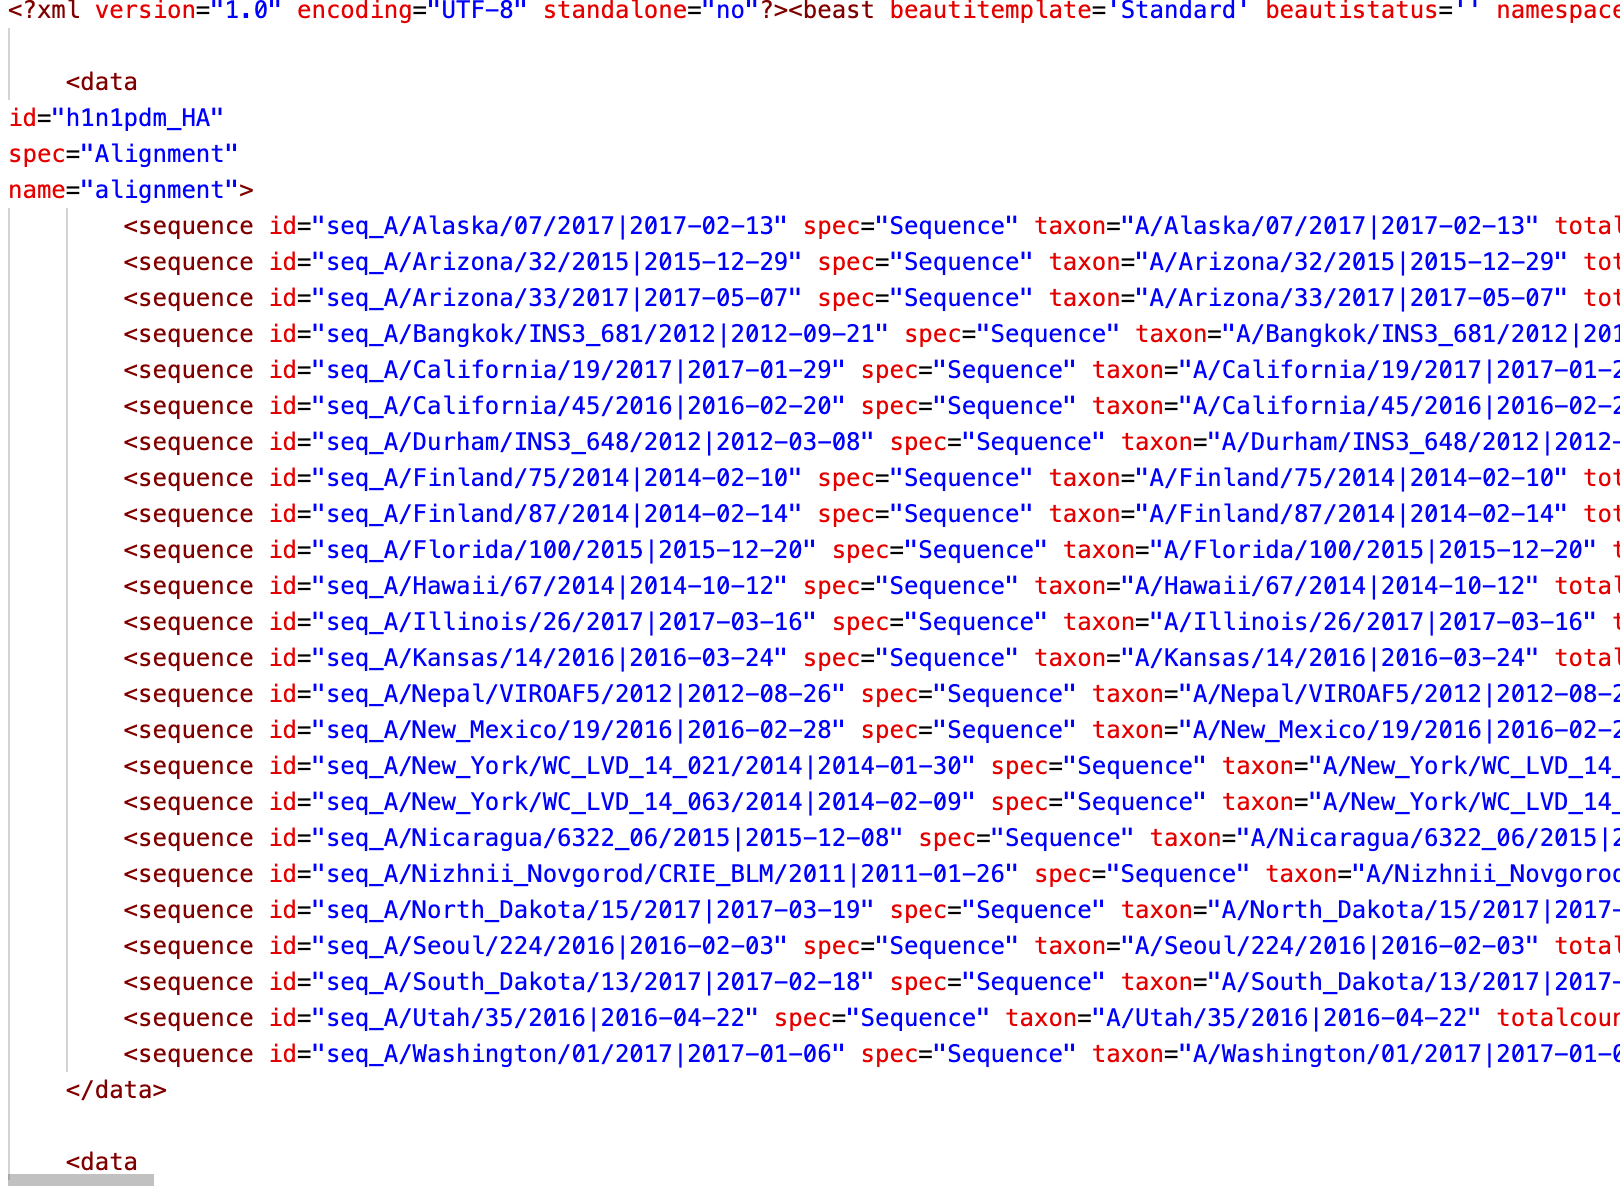
\includegraphics[width=1\textwidth]{figures/Datalook.png}
    \caption{A first look at the xml.}
    \label{fig:example1}
\end{figure}

After opening the xml, we can scroll down to have a look at the settings of the analyses.
The length of the MCMC chain can be found on the following line.

\begin{lstlisting}[language=XML]
  <run id="mcmc" spec="MCMC" chainLength="10">
\end{lstlisting}

At the moment, the analyses will only run for 10 iteartions, which is nowhere near enough for this analysis, so let's go ahead and up it to 10000000.
Let's scroll to the end of the file where it says:

\begin{lstlisting}[language=XML]
  <logger id="tracelog" spec="Logger" fileName="$(filebase).log" logEvery="1000" model="@posterior" sanitiseHeaders="true" sort="smart">
  <log idref="posterior"/>
  <log idref="likelihood"/>
  <log idref="prior"/>
  <log idref="treeLikelihood.h1n1pdm_HA"/>
  <log id="TreeHeight.t:h1n1pdm_HA" spec="beast.base.evolution.tree.TreeStatLogger" tree="@Tree.t:h1n1pdm_HA"/>
  <log idref="treeLikelihood.h1n1pdm_NA"/>
  <log id="TreeHeight.t:h1n1pdm_NA" spec="beast.base.evolution.tree.TreeStatLogger" tree="@Tree.t:h1n1pdm_NA"/>
  <log idref="clockRate.c:h1n1pdm_NA"/>
  <log idref="clockRate.c:h1n1pdm_HA"/>
  <log idref="kappa.s:h1n1pdm_HA"/>
  <log idref="freqParameter.s:h1n1pdm_HA"/>
  <log idref="freqParameter.s:h1n1pdm_NA"/>
  <log idref="kappa.s:h1n1pdm_NA"/>
  <log idref="popSize.t:h1n1pdm_HA"/>
  <log idref="CoalescentConstant.t:h1n1pdm_HA"/>
  <log idref="popSize.t:h1n1pdm_NA"/>
  <log idref="CoalescentConstant.t:h1n1pdm_NA"/>
</logger>
<logger id="screenlog" spec="Logger" logEvery="1000">
  <log idref="posterior"/>
  <log idref="likelihood"/>
  <log idref="prior"/>
</logger>
<logger id="treelog.t:h1n1pdm_HA" spec="Logger" fileName="$(filebase)-$(tree).trees" logEvery="10000000" mode="tree">
  <log id="TreeWithMetaDataLogger.t:h1n1pdm_HA" spec="beast.base.evolution.TreeWithMetaDataLogger" tree="@Tree.t:h1n1pdm_HA"/>
</logger>
<logger id="treelog.t:h1n1pdm_NA" spec="Logger" fileName="$(filebase)-$(tree).trees" logEvery="1000" mode="tree">
  <log id="TreeWithMetaDataLogger.t:h1n1pdm_NA" spec="beast.base.evolution.TreeWithMetaDataLogger" tree="@Tree.t:h1n1pdm_NA"/>
</logger>
<operatorschedule id="OperatorSchedule" spec="OperatorSchedule"/>
\end{lstlisting}

This part of the code says that we are logging 3 files, one log files (with all the parameters) and 2 trees files, one for each alignment.
It also specifies how often each of these files is logged.
For each file, a filename is specified, $\$(filebase)$ means that beast logs to the file with the same name as the xml.
$\$(tree)$ uses the id of the tree that is being logged in the filename.
To reduce the length of the filename, we can change the filenames, for example to:

\begin{lstlisting}[language=XML]
<logger id="treelog.t:h1n1pdm_HA" spec="Logger" fileName="$(filebase)-HA.trees" logEvery="10000000" mode="tree">
  <log id="TreeWithMetaDataLogger.t:h1n1pdm_HA" spec="beast.base.evolution.TreeWithMetaDataLogger" tree="@Tree.t:h1n1pdm_HA"/>
</logger>
<logger id="treelog.t:h1n1pdm_NA" spec="Logger" fileName="$(filebase)-NA.trees" logEvery="1000" mode="tree">
  <log id="TreeWithMetaDataLogger.t:h1n1pdm_NA" spec="beast.base.evolution.TreeWithMetaDataLogger" tree="@Tree.t:h1n1pdm_NA"/>
</logger>
\end{lstlisting}

Does anything seem odd in how the files will be logged?
If so, make the change.


If you want to make sure that none of the changes broke the xml, we can save the changes and start the run in BEAST.
If the run starts and logs the correct file names.
The run proceeds oddly fast, however.
Let's open the log file in Tracer and see if we can spot what is going wrong.

 
\begin{figure}[H]
  \centering
  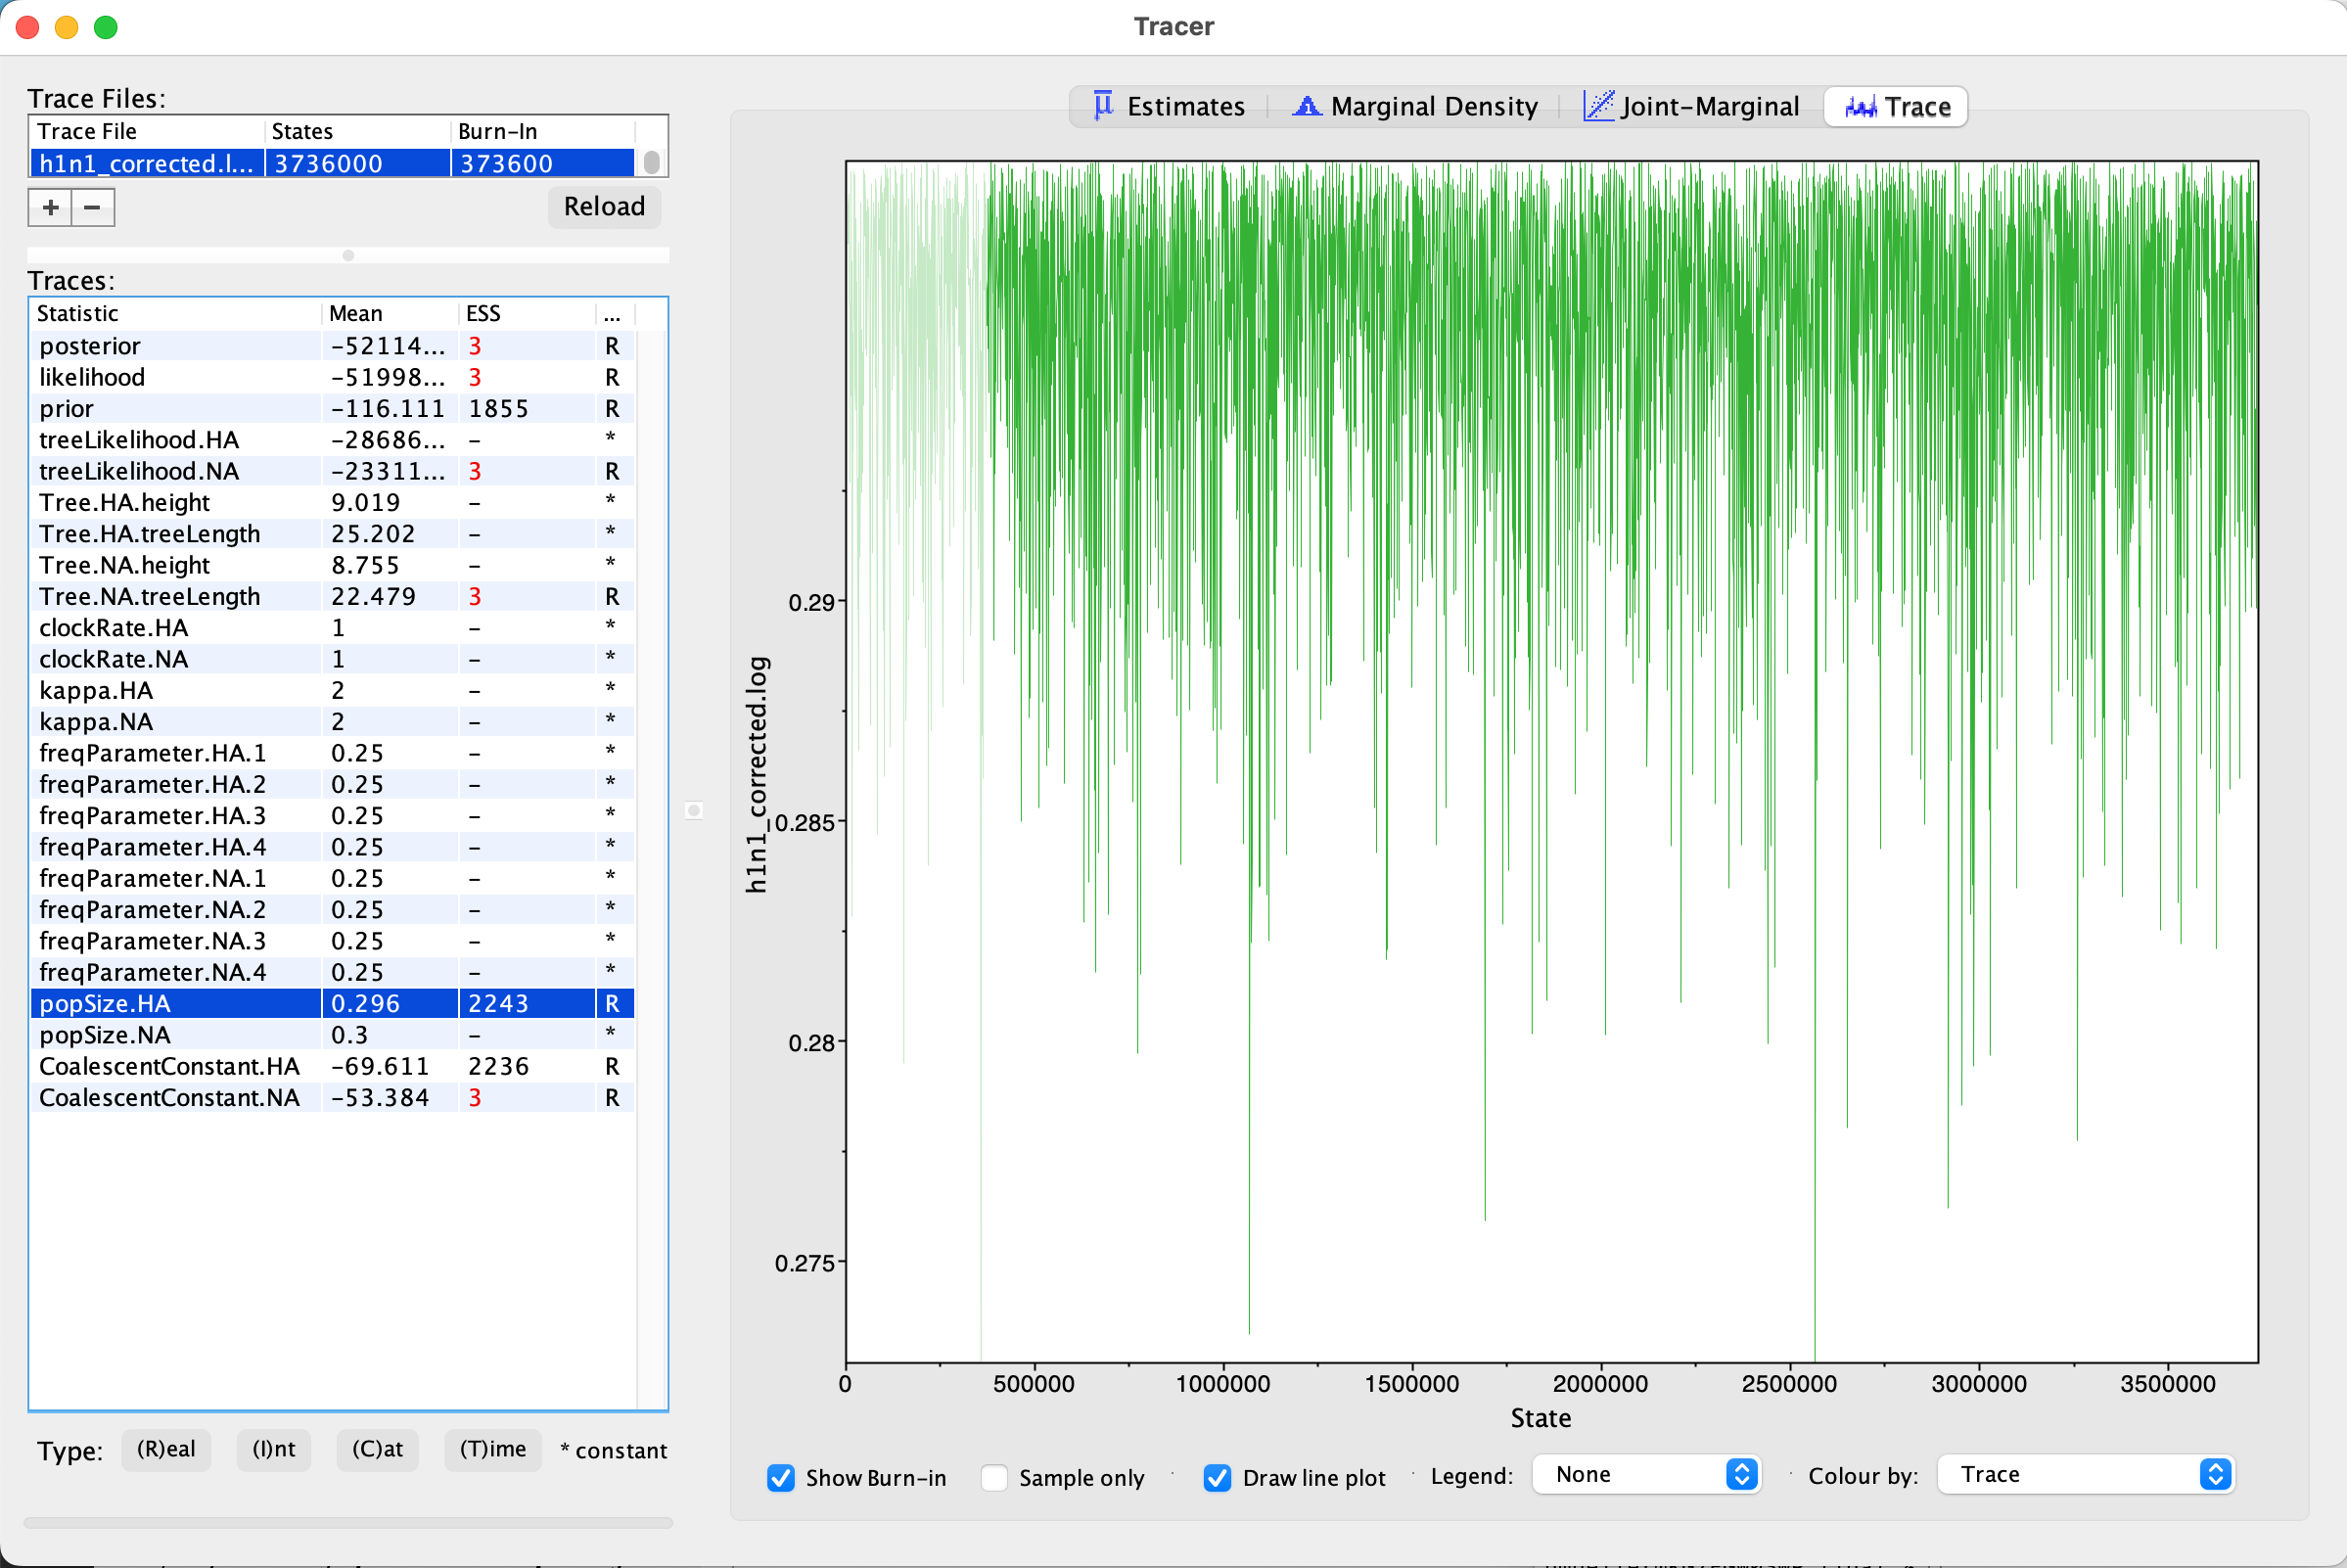
\includegraphics[width=0.5\textwidth]{figures/Tracer.png}
  \caption{Only one of the $popSize.t:h1n1pdm\_HA$ is being explored.}
  \label{fig:example1}
\end{figure}


Since only one of the pop sizes parameters is being explored, something is probably wrong in the settings of the xml.
Additionally, the pop size parameter seems to hit some wall at 0.3 where it's blocked.
Let's see if we can find out what is going on.

Let's go back to the xml and search for all the places where $popSize.t:h1n1pdm\_HA$ shows up.
First, we see it in the state block. 
Can you spot why the parameter is hitting a wall at 0.3?

\begin{lstlisting}[language=XML]
<parameter id="clockRate.c:h1n1pdm_NA" spec="parameter.RealParameter" lower="0.0" name="stateNode">1.0</parameter>
<parameter id="clockRate.c:h1n1pdm_HA" spec="parameter.RealParameter" lower="0.0" name="stateNode">1.0</parameter>
<parameter id="kappa.s:h1n1pdm_HA" spec="parameter.RealParameter" lower="0.0" name="stateNode">2.0</parameter>
<parameter id="freqParameter.s:h1n1pdm_HA" spec="parameter.RealParameter" dimension="4" lower="0.0" name="stateNode" upper="1.0">0.25</parameter>
<parameter id="freqParameter.s:h1n1pdm_NA" spec="parameter.RealParameter" dimension="4" lower="0.0" name="stateNode" upper="1.0">0.25</parameter>
<parameter id="kappa.s:h1n1pdm_NA" spec="parameter.RealParameter" lower="0.0" name="stateNode">2.0</parameter>
<parameter id="popSize.t:h1n1pdm_HA" spec="parameter.RealParameter" lower="0.0" name="stateNode" upper="0.3">0.1</parameter>
<parameter id="popSize.t:h1n1pdm_NA" spec="parameter.RealParameter" lower="0.0" name="stateNode">0.3</parameter>
</state>
\end{lstlisting}

Let's see where else the parameter shows up.
In the operator block of each xml, we specify which MCMC operations can occur.
We have one operator acting on the parameter $popSize.t:h1n1pdm\_HA$. 


\begin{lstlisting}[language=XML]
<operator id="CoalescentConstantNarrow.t:h1n1pdm_HA" spec="Exchange" tree="@Tree.t:h1n1pdm_HA" weight="15.0"/>
<operator id="CoalescentConstantWide.t:h1n1pdm_HA" spec="Exchange" isNarrow="false" tree="@Tree.t:h1n1pdm_HA" weight="3.0"/>
<operator id="CoalescentConstantWilsonBalding.t:h1n1pdm_HA" spec="WilsonBalding" tree="@Tree.t:h1n1pdm_HA" weight="3.0"/>
<operator id="PopSizeScaler.t:h1n1pdm_HA" spec="kernel.BactrianScaleOperator" parameter="@popSize.t:h1n1pdm_HA" upper="10.0" weight="100000000.0"/>
<operator id="CoalescentConstantBICEPSEpochTop.t:h1n1pdm_NA" spec="EpochFlexOperator" scaleFactor="0.1" tree="@Tree.t:h1n1pdm_NA" weight="2.0"/>
<operator id="CoalescentConstantBICEPSEpochAll.t:h1n1pdm_NA" spec="EpochFlexOperator" fromOldestTipOnly="false" scaleFactor="0.1" tree="@Tree.t:h1n1pdm_NA" weight="2.0"/>
\end{lstlisting}

Oddly that operator has weigth 100000000.
BEAST will use one operator per iteration in the MCMC. 
The chance of this operator being called is given by its relative weight.
100000000 means that BEAST will essentially only use this one operator and ignore all others.
Let's change it to 3 (the default for this operator) and try running the file again.
(Pro tip: it's a lot faster to start a run from the Terminal instead of using the GUI of BEAST).

After a few iterations, we can reload the log file in Tracer and confirm that all the values change over the course of the MCMC.



\hypertarget{Changing priors}{%
\section{Changing priors}\label{changing-priors}}
If I just want to change some of my priors in the xml, it's often easier to do that directly in the xml instead of loading things in BEAUti or setting up everything from scratch.

In the xml, there is an entire block that is called prior

\begin{lstlisting}[language=XML]
<distribution id="prior" spec="CompoundDistribution">
<distribution id="CoalescentConstant.t:h1n1pdm_HA" spec="Coalescent">
    <populationModel id="ConstantPopulation.t:h1n1pdm_HA" spec="ConstantPopulation" popSize="@popSize.t:h1n1pdm_HA"/>
    <treeIntervals id="TreeIntervals.t:h1n1pdm_HA" spec="beast.base.evolution.tree.TreeIntervals" tree="@Tree.t:h1n1pdm_HA"/>
</distribution>
<distribution id="CoalescentConstant.t:h1n1pdm_NA" spec="Coalescent">
    <populationModel id="ConstantPopulation.t:h1n1pdm_NA" spec="ConstantPopulation" popSize="@popSize.t:h1n1pdm_NA"/>
    <treeIntervals id="TreeIntervals.t:h1n1pdm_NA" spec="beast.base.evolution.tree.TreeIntervals" tree="@Tree.t:h1n1pdm_NA"/>
</distribution>
<prior id="ClockPrior.c:h1n1pdm_HA" name="distribution" x="@clockRate.c:h1n1pdm_HA">
    <Uniform id="Uniform.0" name="distr" upper="Infinity"/>
</prior>
<prior id="ClockPrior.c:h1n1pdm_NA" name="distribution" x="@clockRate.c:h1n1pdm_NA">
    <Uniform id="Uniform.3" name="distr" upper="Infinity"/>
</prior>
<prior id="FrequenciesPrior.s:h1n1pdm_HA" name="distribution" x="@freqParameter.s:h1n1pdm_HA">
    <distr id="Dirichlet.0" spec="distribution.Dirichlet">
        <parameter id="RealParameter.4" spec="parameter.RealParameter" dimension="4" estimate="false" name="alpha">4.0 4.0 4.0 4.0</parameter>
    </distr>
</prior>
<prior id="FrequenciesPrior.s:h1n1pdm_NA" name="distribution" x="@freqParameter.s:h1n1pdm_NA">
    <distr id="Dirichlet.0.h1n1pdm_NA" spec="distribution.Dirichlet">
        <parameter id="RealParameter.4.h1n1pdm_NA" spec="parameter.RealParameter" dimension="4" estimate="false" name="alpha">4.0 4.0 4.0 4.0</parameter>
    </distr>
</prior>
<prior id="KappaPrior.s:h1n1pdm_HA" name="distribution" x="@kappa.s:h1n1pdm_HA">
    <LogNormal id="LogNormalDistributionModel.0" name="distr">
        <parameter id="RealParameter.2" spec="parameter.RealParameter" estimate="false" name="M">1.0</parameter>
        <parameter id="RealParameter.3" spec="parameter.RealParameter" estimate="false" name="S">1.25</parameter>
    </LogNormal>
</prior>
<prior id="KappaPrior.s:h1n1pdm_NA" name="distribution" x="@kappa.s:h1n1pdm_NA">
    <LogNormal id="LogNormalDistributionModel.0.h1n1pdm_NA" name="distr">
        <parameter id="RealParameter.2.h1n1pdm_NA" spec="parameter.RealParameter" estimate="false" name="M">1.0</parameter>
        <parameter id="RealParameter.3.h1n1pdm_NA" spec="parameter.RealParameter" estimate="false" name="S">1.25</parameter>
    </LogNormal>
</prior>
<prior id="PopSizePrior.t:h1n1pdm_HA" name="distribution" x="@popSize.t:h1n1pdm_HA">
    <OneOnX id="OneOnX.2" name="distr"/>
</prior>
<prior id="PopSizePrior.t:h1n1pdm_NA" name="distribution" x="@popSize.t:h1n1pdm_NA">
    <OneOnX id="OneOnX.3" name="distr"/>
</prior>
</distribution>
\end{lstlisting}

the x=... gives you which parameter the prior is on.
The prior distribution for the parameter $popSize.t:h1n1pdm\_HA$ is currently OneOnX, which is an inverse uniform distribution.
Let's assume we have some more information about that prior and we know a lognormal distribution with M="2" and S="1" is a better representation of our prior knowledge of that parameter.
To change the prior distribution, we can replace the prior on $popSize.t:h1n1pdm\_HA$ with the below xml part.

\begin{lstlisting}[language=XML]
<prior id="PopSizePrior.t:h1n1pdm_HA" name="distribution" x="@popSize.t:h1n1pdm_HA">
    <LogNormal id="OneOnX.2" name="distr" M="2" S="1"/>
</prior>
\end{lstlisting}
Note that the id of the distribution is still OneOnX.2. 
The id of an xml object however doesn't matter with regards to what the object does.

\hypertarget{Linking parameters}{%
\section{Linking parameters}\label{linking-parameters}}

Sometimes, we want to be able to link parameters in different parts of the xml.
For example, the same population level process gave rise to the HA and NA segments, so we might want to link the population size parameters of the two segments.
We can do that directly in the xml.

At the moment, we have two tree priors, one for each segment.
The tree priors are constant population coalescent priors, and there is one for each tree.
In the xml, the tree priors are specified as follows:

\begin{lstlisting}[language=XML]
<distribution id="CoalescentConstant.t:h1n1pdm_HA" spec="Coalescent">
<populationModel id="ConstantPopulation.t:h1n1pdm_HA" spec="ConstantPopulation" popSize="@popSize.t:h1n1pdm_HA"/>
<treeIntervals id="TreeIntervals.t:h1n1pdm_HA" spec="beast.base.evolution.tree.TreeIntervals" tree="@Tree.t:h1n1pdm_HA"/>
</distribution>
<distribution id="CoalescentConstant.t:h1n1pdm_NA" spec="Coalescent">
<populationModel id="ConstantPopulation.t:h1n1pdm_NA" spec="ConstantPopulation" popSize="@popSize.t:h1n1pdm_NA"/>
<treeIntervals id="TreeIntervals.t:h1n1pdm_NA" spec="beast.base.evolution.tree.TreeIntervals" tree="@Tree.t:h1n1pdm_NA"/>
</distribution>
\end{lstlisting}

How do we link the two population size parameters?
We can simply replace the population size parameter of one of the tree priors with the parameter of the other tree prior.
Let's replace the population size parameter of the NA segment with the population size parameter of the HA segment.

\begin{lstlisting}[language=XML]
  <distribution id="CoalescentConstant.t:h1n1pdm_HA" spec="Coalescent">
  <populationModel id="ConstantPopulation.t:h1n1pdm_HA" spec="ConstantPopulation" popSize="@popSize.t:h1n1pdm_HA"/>
  <treeIntervals id="TreeIntervals.t:h1n1pdm_HA" spec="beast.base.evolution.tree.TreeIntervals" tree="@Tree.t:h1n1pdm_HA"/>
  </distribution>
  <distribution id="CoalescentConstant.t:h1n1pdm_NA" spec="Coalescent">
  <populationModel id="ConstantPopulation.t:h1n1pdm_NA" spec="ConstantPopulation" popSize="@popSize.t:h1n1pdm_HA"/>
  <treeIntervals id="TreeIntervals.t:h1n1pdm_NA" spec="beast.base.evolution.tree.TreeIntervals" tree="@Tree.t:h1n1pdm_NA"/>
  </distribution>
\end{lstlisting}
  
Now, $CoalescentConstant.t:h1n1pdm\_NA$, the tree prior on the NA segment, uses the population size parameter of the HA segment.
Essentially, we are done now.
However, the parameter $popSize.t:h1n1pdm\_NA$ is still in the xml, and it is still being explored.
We can remove it from the xml, and BEAST will no longer explore it.
Let's remove it from the state block.

\begin{lstlisting}[language=XML]
  <parameter id="kappa.s:h1n1pdm_NA" spec="parameter.RealParameter" lower="0.0" name="stateNode">2.0</parameter>
  <parameter id="popSize.t:h1n1pdm_HA" spec="parameter.RealParameter" lower="0.0" name="stateNode" upper="3">0.1</parameter>
  <parameter id="popSize.t:h1n1pdm_NA" spec="parameter.RealParameter" lower="0.0" name="stateNode">0.3</parameter>
</state>
\end{lstlisting}

Next, we have to remove it from the priors block
\begin{lstlisting}[language=XML]
  <prior id="PopSizePrior.t:h1n1pdm_HA" name="distribution" x="@popSize.t:h1n1pdm_HA">
      <OneOnX id="OneOnX.2" name="distr"/>
  </prior>
  <prior id="PopSizePrior.t:h1n1pdm_NA" name="distribution" x="@popSize.t:h1n1pdm_NA">
      <OneOnX id="OneOnX.3" name="distr"/>
  </prior>
</distribution>
\end{lstlisting}
Then, we can remove it from the operators block.

\begin{lstlisting}[language=XML]
<operator id="PopSizeScaler.t:h1n1pdm_HA" spec="kernel.BactrianScaleOperator" parameter="@popSize.t:h1n1pdm_HA" upper="10.0" weight="3.0"/>
<operator id="CoalescentConstantBICEPSEpochTop.t:h1n1pdm_NA" spec="EpochFlexOperator" scaleFactor="0.1" tree="@Tree.t:h1n1pdm_NA" weight="2.0"/>
<operator id="CoalescentConstantBICEPSEpochAll.t:h1n1pdm_NA" spec="EpochFlexOperator" fromOldestTipOnly="false" scaleFactor="0.1" tree="@Tree.t:h1n1pdm_NA" weight="2.0"/>
<operator id="CoalescentConstantBICEPSTreeFlex.t:h1n1pdm_NA" spec="TreeStretchOperator" scaleFactor="0.01" tree="@Tree.t:h1n1pdm_NA" weight="2.0"/>
<operator id="CoalescentConstantTreeRootScaler.t:h1n1pdm_NA" spec="kernel.BactrianScaleOperator" rootOnly="true" scaleFactor="0.1" tree="@Tree.t:h1n1pdm_NA" upper="10.0" weight="3.0"/>
<operator id="CoalescentConstantUniformOperator.t:h1n1pdm_NA" spec="kernel.BactrianNodeOperator" tree="@Tree.t:h1n1pdm_NA" weight="30.0"/>
<operator id="CoalescentConstantSubtreeSlide.t:h1n1pdm_NA" spec="kernel.BactrianSubtreeSlide" tree="@Tree.t:h1n1pdm_NA" weight="15.0"/>
<operator id="CoalescentConstantNarrow.t:h1n1pdm_NA" spec="Exchange" tree="@Tree.t:h1n1pdm_NA" weight="15.0"/>
<operator id="CoalescentConstantWide.t:h1n1pdm_NA" spec="Exchange" isNarrow="false" tree="@Tree.t:h1n1pdm_NA" weight="3.0"/>
<operator id="CoalescentConstantWilsonBalding.t:h1n1pdm_NA" spec="WilsonBalding" tree="@Tree.t:h1n1pdm_NA" weight="3.0"/>
<operator id="PopSizeScaler.t:h1n1pdm_NA" spec="kernel.BactrianScaleOperator" parameter="@popSize.t:h1n1pdm_NA" upper="10.0" weight="3.0"/>
\end{lstlisting}

Parameters can have multiple operators, for example, the tree parameters have multiple operators acting on the tree.
Removing just one of them will not fix this parameter.


And, lastly, we have to keep the parameter from being logged to a file.

\begin{lstlisting}[language=XML]
<log idref="kappa.s:h1n1pdm_HA"/>
<log idref="freqParameter.s:h1n1pdm_HA"/>
<log idref="freqParameter.s:h1n1pdm_NA"/>
<log idref="kappa.s:h1n1pdm_NA"/>
<log idref="popSize.t:h1n1pdm_HA"/>
<log idref="CoalescentConstant.t:h1n1pdm_HA"/>
<log idref="popSize.t:h1n1pdm_NA"/>
<log idref="CoalescentConstant.t:h1n1pdm_NA"/>
</logger>
\end{lstlisting}

Now, the parameter $popSize.t:h1n1pdm_NA$ is no longer in the xml, and BEAST will no longer explore it.
We could have removed it from the MCMC by only changing the xml at two points, how?

\hypertarget{Fixing parameters}{%
\section{Fixing parameters}\label{Fixing-parameters}}
Fixing parameter is rather simple.
The intial value of each parameter is given by its value in the state block.
Let's say we know the clock rate of the HA segment is 0.005.
We can fix the clock rate of the HA segment by changing the xml as follows:
\begin{lstlisting}[language=XML]
<parameter id="clockRate.c:h1n1pdm_NA" spec="parameter.RealParameter" lower="0.0" name="stateNode">1.0</parameter>
\end{lstlisting}
to 
\begin{lstlisting}[language=XML]
  <parameter id="clockRate.c:h1n1pdm_NA" spec="parameter.RealParameter" lower="0.0" name="stateNode">0.005</parameter>
\end{lstlisting}

The parameter $clockRate.c:h1n1pdm\_NA$ is now initalized to 0.005 but will still be explored by the MCMC.
To fix the parameter, we have to remove all operators acting on the parameter.
Let's move to the operators block and search for $clockRate.c:h1n1pdm\_NA$

The operators acting on the parameter are:
\begin{lstlisting}[language=XML]
  <operator id="StrictClockRateScaler.c:h1n1pdm_HA" spec="AdaptableOperatorSampler" weight="1.5">
  <parameter idref="clockRate.c:h1n1pdm_HA"/>
  <operator id="AVMNOperator.h1n1pdm_HA" spec="kernel.AdaptableVarianceMultivariateNormalOperator" allowNonsense="true" beta="0.05" burnin="400" initial="800" weight="0.1">
      <transformations id="AVMNSumTransform.h1n1pdm_HA" spec="operator.kernel.Transform$LogConstrainedSumTransform">
          <f idref="freqParameter.s:h1n1pdm_HA"/>
      </transformations>
      <transformations id="AVMNLogTransform.h1n1pdm_HA" spec="operator.kernel.Transform$LogTransform">
          <f idref="clockRate.c:h1n1pdm_HA"/>
          <f idref="kappa.s:h1n1pdm_HA"/>
      </transformations>
      <transformations id="AVMNNoTransform.h1n1pdm_HA" spec="operator.kernel.Transform$NoTransform">
          <f idref="Tree.t:h1n1pdm_HA"/>
      </transformations>
  </operator>
  <operator id="StrictClockRateScalerX.c:h1n1pdm_HA" spec="kernel.BactrianScaleOperator" parameter="@clockRate.c:h1n1pdm_HA" upper="10.0" weight="3.0"/>
</operator>
<operator id="strictClockUpDownOperator.c:h1n1pdm_HA" spec="AdaptableOperatorSampler" weight="1.5">
  <parameter idref="clockRate.c:h1n1pdm_HA"/>
  <tree idref="Tree.t:h1n1pdm_HA"/>
  <operator idref="AVMNOperator.h1n1pdm_HA"/>
  <operator id="strictClockUpDownOperatorX.c:h1n1pdm_HA" spec="operator.kernel.BactrianUpDownOperator" scaleFactor="0.75" weight="3.0">
      <up idref="clockRate.c:h1n1pdm_HA"/>
      <down idref="Tree.t:h1n1pdm_HA"/>
  </operator>
</operator>
\end{lstlisting}

We could just remove these lines, but then all other operators that reference the following would fail.

\begin{lstlisting}[language=XML]
<operator id="AVMNOperator.h1n1pdm_HA" spec="kernel.AdaptableVarianceMultivariateNormalOperator" allowNonsense="true" beta="0.05" burnin="400" initial="800" weight="0.1">
<transformations id="AVMNSumTransform.h1n1pdm_HA" spec="operator.kernel.Transform$LogConstrainedSumTransform">
    <f idref="freqParameter.s:h1n1pdm_HA"/>
</transformations>
<transformations id="AVMNLogTransform.h1n1pdm_HA" spec="operator.kernel.Transform$LogTransform">
    <f idref="clockRate.c:h1n1pdm_HA"/>
    <f idref="kappa.s:h1n1pdm_HA"/>
</transformations>
<transformations id="AVMNNoTransform.h1n1pdm_HA" spec="operator.kernel.Transform$NoTransform">
    <f idref="Tree.t:h1n1pdm_HA"/>
</transformations>
</operator>
\end{lstlisting}

To prevent that, we can remove the clock rate from the block.

\begin{lstlisting}[language=XML]
  <operator id="AVMNOperator.h1n1pdm_HA" spec="kernel.AdaptableVarianceMultivariateNormalOperator" allowNonsense="true" beta="0.05" burnin="400" initial="800" weight="0.1">
  <transformations id="AVMNSumTransform.h1n1pdm_HA" spec="operator.kernel.Transform$LogConstrainedSumTransform">
      <f idref="freqParameter.s:h1n1pdm_HA"/>
  </transformations>
  <transformations id="AVMNLogTransform.h1n1pdm_HA" spec="operator.kernel.Transform$LogTransform">
      <f idref="kappa.s:h1n1pdm_HA"/>
  </transformations>
  <transformations id="AVMNNoTransform.h1n1pdm_HA" spec="operator.kernel.Transform$NoTransform">
      <f idref="Tree.t:h1n1pdm_HA"/>
  </transformations>
  </operator>
\end{lstlisting}

And put this block instead in the next operator where it was previously referenced with idref.
This is the case for the KappaScaler:

\begin{lstlisting}[language=XML]
<operator id="KappaScaler.s:h1n1pdm_HA" spec="AdaptableOperatorSampler" weight="0.05">
<parameter idref="kappa.s:h1n1pdm_HA"/>
<operator idref="AVMNOperator.h1n1pdm_HA"/>
<operator id="KappaScalerX.s:h1n1pdm_HA" spec="kernel.BactrianScaleOperator" parameter="@kappa.s:h1n1pdm_HA" scaleFactor="0.1" upper="10.0" weight="0.1"/>
</operator>
\end{lstlisting}


We can now make sure that the $AVMNOperator.h1n1pdm\_HA$ is properly initialized here instead.
\begin{lstlisting}[language=XML]
<operator id="KappaScaler.s:h1n1pdm_HA" spec="AdaptableOperatorSampler" weight="0.05">
<parameter idref="kappa.s:h1n1pdm_HA"/>
<operator id="AVMNOperator.h1n1pdm_HA" spec="kernel.AdaptableVarianceMultivariateNormalOperator" allowNonsense="true" beta="0.05" burnin="400" initial="800" weight="0.1">
    <transformations id="AVMNSumTransform.h1n1pdm_HA" spec="operator.kernel.Transform$LogConstrainedSumTransform">
        <f idref="freqParameter.s:h1n1pdm_HA"/>
    </transformations>
    <transformations id="AVMNLogTransform.h1n1pdm_HA" spec="operator.kernel.Transform$LogTransform">
        <f idref="kappa.s:h1n1pdm_HA"/>
    </transformations>
    <transformations id="AVMNNoTransform.h1n1pdm_HA" spec="operator.kernel.Transform$NoTransform">
        <f idref="Tree.t:h1n1pdm_HA"/>
    </transformations>
</operator>
<operator id="KappaScalerX.s:h1n1pdm_HA" spec="kernel.BactrianScaleOperator" parameter="@kappa.s:h1n1pdm_HA" scaleFactor="0.1" upper="10.0" weight="0.1"/>
</operator>
\end{lstlisting}

When we now run the xml in beast, the clock rate of the HA segment is fixed to 0.005.


\begin{itemize}
\item
  \href{http://www.beast2.org/book.html}{Bayesian Evolutionary Analysis
  with BEAST 2} \citep{BEAST2book2014}
\item
  BEAST 2 website and documentation: \url{http://www.beast2.org/}
\item
  Join the BEAST user discussion:
  \url{http://groups.google.com/group/beast-users} \clearpage
\end{itemize}

\printbibliography[heading=relevref]
\end{document}
